% Hand-written TikZ — tactic taxonomy as a 3-column card grid (portrait-friendly).
% Each card = one family, with its tactics as bulleted items inside.
% Designed to fit \textwidth without scaling and never clip at page edges.
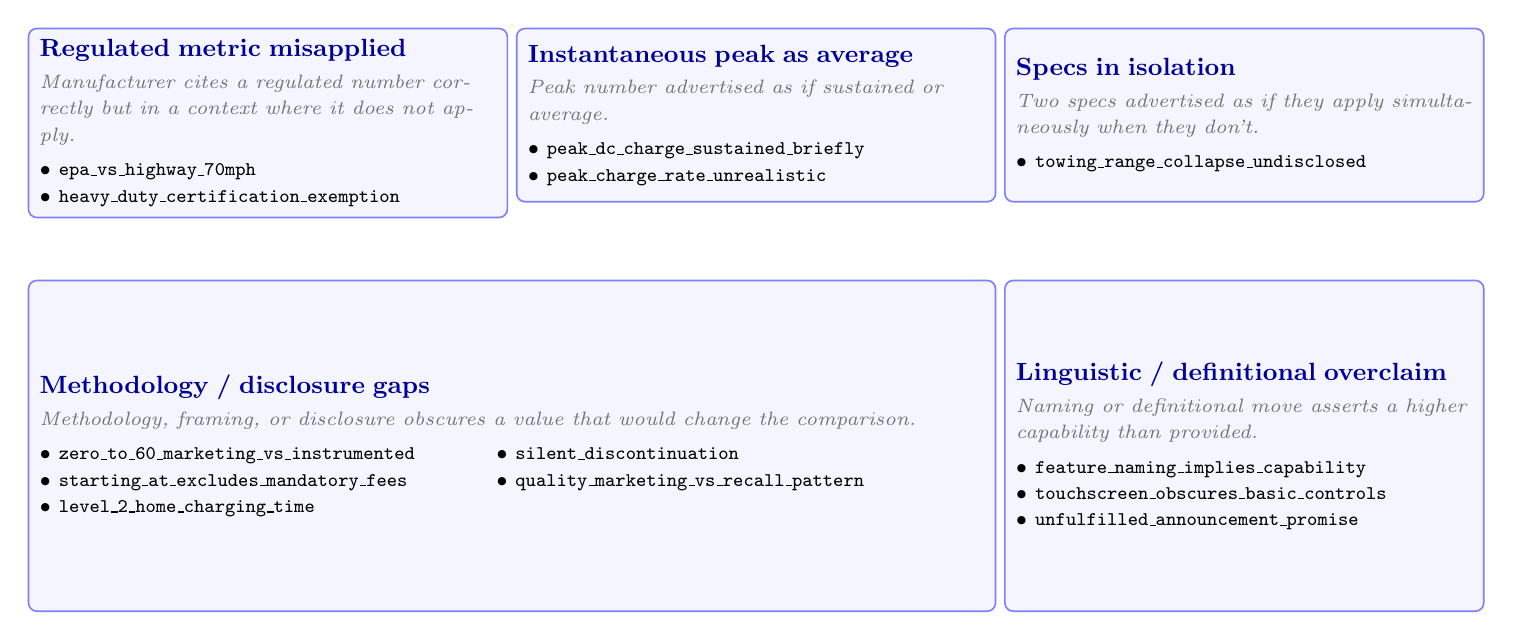
\begin{tikzpicture}[
    every node/.style={font=\footnotesize, align=left},
    card/.style={
      draw, rounded corners=3pt, line width=0.6pt,
      fill=blue!4, draw=blue!50,
      inner sep=4pt, outer sep=0pt,
      text width=58mm, minimum height=22mm,
    },
  ]
% --- column x-positions
\def\cA{0}
\def\cB{62mm}
\def\cC{124mm}
% --- row y-positions
\def\rA{0}
\def\rB{-32mm}

% Row 1, Col 1 — Regulated metric misapplied (2 tactics)
\node[card, anchor=north west] at (\cA, \rA) {%
  {\bfseries\small\color{blue!60!black} Regulated metric misapplied}\\[2pt]
  {\scriptsize\itshape\color{black!55} Manufacturer cites a regulated number correctly but in a context where it does not apply.}\\[3pt]
  {\scriptsize\ttfamily $\bullet$ epa\_vs\_highway\_70mph}\\
  {\scriptsize\ttfamily $\bullet$ heavy\_duty\_certification\_exemption}%
};

% Row 1, Col 2 — Instantaneous peak as average (2 tactics)
\node[card, anchor=north west] at (\cB, \rA) {%
  {\bfseries\small\color{blue!60!black} Instantaneous peak as average}\\[2pt]
  {\scriptsize\itshape\color{black!55} Peak number advertised as if sustained or average.}\\[3pt]
  {\scriptsize\ttfamily $\bullet$ peak\_dc\_charge\_sustained\_briefly}\\
  {\scriptsize\ttfamily $\bullet$ peak\_charge\_rate\_unrealistic}%
};

% Row 1, Col 3 — Specs in isolation (1 tactic)
\node[card, anchor=north west] at (\cC, \rA) {%
  {\bfseries\small\color{blue!60!black} Specs in isolation}\\[2pt]
  {\scriptsize\itshape\color{black!55} Two specs advertised as if they apply simultaneously when they don't.}\\[3pt]
  {\scriptsize\ttfamily $\bullet$ towing\_range\_collapse\_undisclosed}%
};

% Row 2, Cols 1+2 (spans 2 cols) — Methodology / disclosure gaps (5 tactics)
\node[card, anchor=north west, text width=120mm, minimum height=42mm] at (\cA, \rB) {%
  {\bfseries\small\color{blue!60!black} Methodology / disclosure gaps}\\[2pt]
  {\scriptsize\itshape\color{black!55} Methodology, framing, or disclosure obscures a value that would change the comparison.}\\[3pt]
  \begin{minipage}[t]{56mm}
    {\scriptsize\ttfamily $\bullet$ zero\_to\_60\_marketing\_vs\_instrumented}\\
    {\scriptsize\ttfamily $\bullet$ starting\_at\_excludes\_mandatory\_fees}\\
    {\scriptsize\ttfamily $\bullet$ level\_2\_home\_charging\_time}
  \end{minipage}\hspace{2mm}%
  \begin{minipage}[t]{58mm}
    {\scriptsize\ttfamily $\bullet$ silent\_discontinuation}\\
    {\scriptsize\ttfamily $\bullet$ quality\_marketing\_vs\_recall\_pattern}
  \end{minipage}%
};

% Row 2, Col 3 — Linguistic / definitional overclaim (3 tactics)
\node[card, anchor=north west, minimum height=42mm] at (\cC, \rB) {%
  {\bfseries\small\color{blue!60!black} Linguistic / definitional overclaim}\\[2pt]
  {\scriptsize\itshape\color{black!55} Naming or definitional move asserts a higher capability than provided.}\\[3pt]
  {\scriptsize\ttfamily $\bullet$ feature\_naming\_implies\_capability}\\
  {\scriptsize\ttfamily $\bullet$ touchscreen\_obscures\_basic\_controls}\\
  {\scriptsize\ttfamily $\bullet$ unfulfilled\_announcement\_promise}%
};
\end{tikzpicture}
